\documentclass{article}
\usepackage[utf8]{inputenc}
\usepackage[colorlinks=true, allcolors=blue]{hyperref}
\usepackage{graphicx}
\usepackage{setspace}
\usepackage{parskip}

\title{Visual Analytics for Big Data (WMCS16000)\\
\large{Assignment 2}}
\author{Shaniya Hassan Ali (s3555496)
\\Carlos Huerta (s3743071) }
\date{September 2018}

\begin{document}

\maketitle

\section{Task	1:	Exploring	the	incidents’	geographical	distribution}
\subsection{Are there high variations of incident densities over Seattle? Which are the low-density zones? Which are the high-density	zones?}
        Incident density over different zones on Seattle vary a lot according to the zone selected, there are zones with lots of criminal activity \textbf{K3} being the maximum which has \textbf{50,487} records of incidents, zones \textbf{M2}, \textbf{K2}, \textbf{M3} and \textbf{E2} have over \textbf{45k} number of records. The low density zones are the zones \textbf{99}, \textbf{O3} and \textbf{Q1} with less than \textbf{19,008} number of records.
        \\
        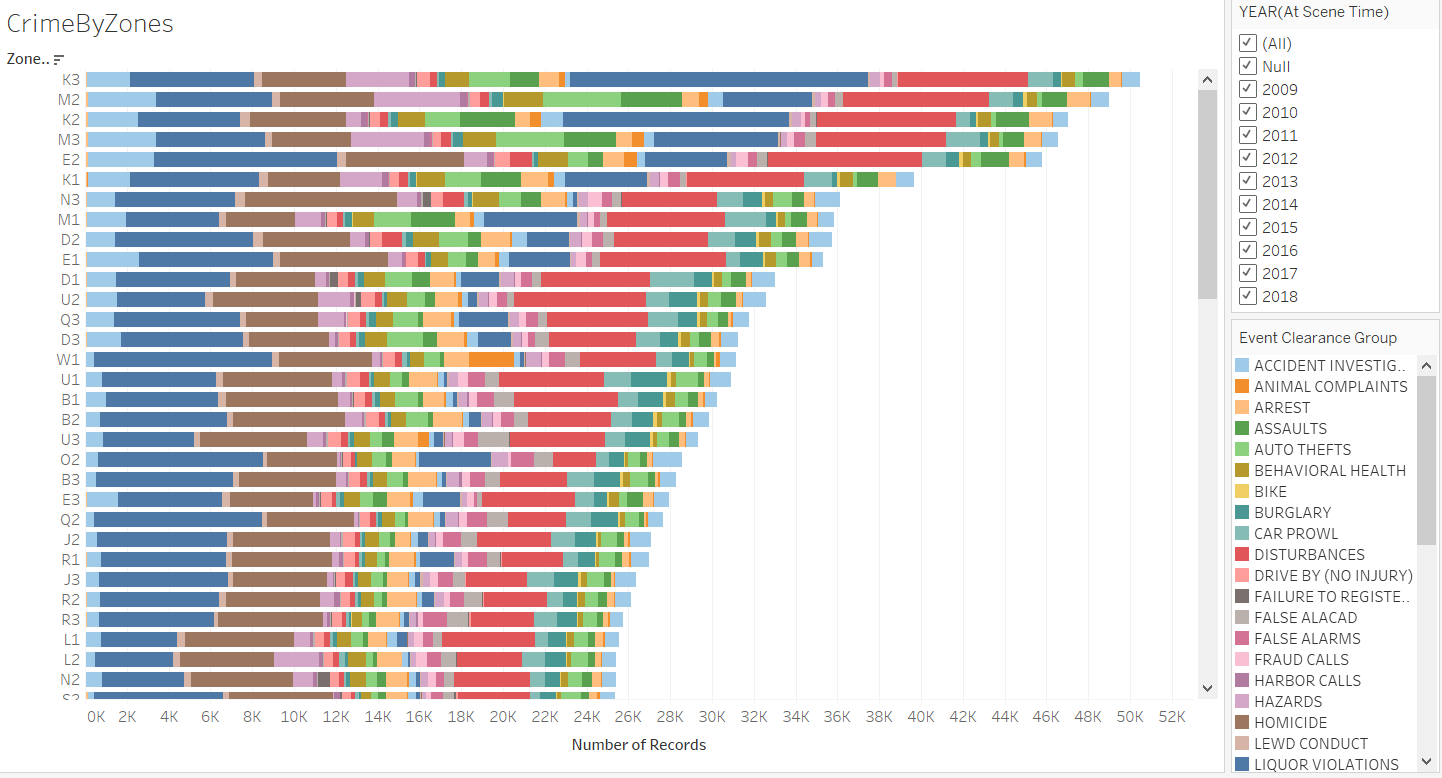
\includegraphics[width=\textwidth]{VisualAnalytics/Assignment2/images/CrimesByZone.PNG}
        \\\\
        The complete visualization can be accesed via tableu public using the following link:
        \url{https://public.tableau.com/profile/charx#!/vizhome/Seattle911Calls_5/CrimeByZones} under metadata and "CrimeByZones" tab.
\subsection{Are there high variations of incident densities over Seattle for	 specific	 types of incidents?	Which	are	these	types	and	which	are	the	variations	you	found?}
    We can observe that the most common type of event are traffic related incidents with nearly \textbf{267k} records, followed by suspicious circumstances with \textbf{222k} records and disturbances with \textbf{200k} records, after that the most reported incident is liquor violations with just \textbf{77k} records. Indeed the majority of the type of the incidents are from the first 3 categories while the other ones don't have a lot of records. 
    \\
    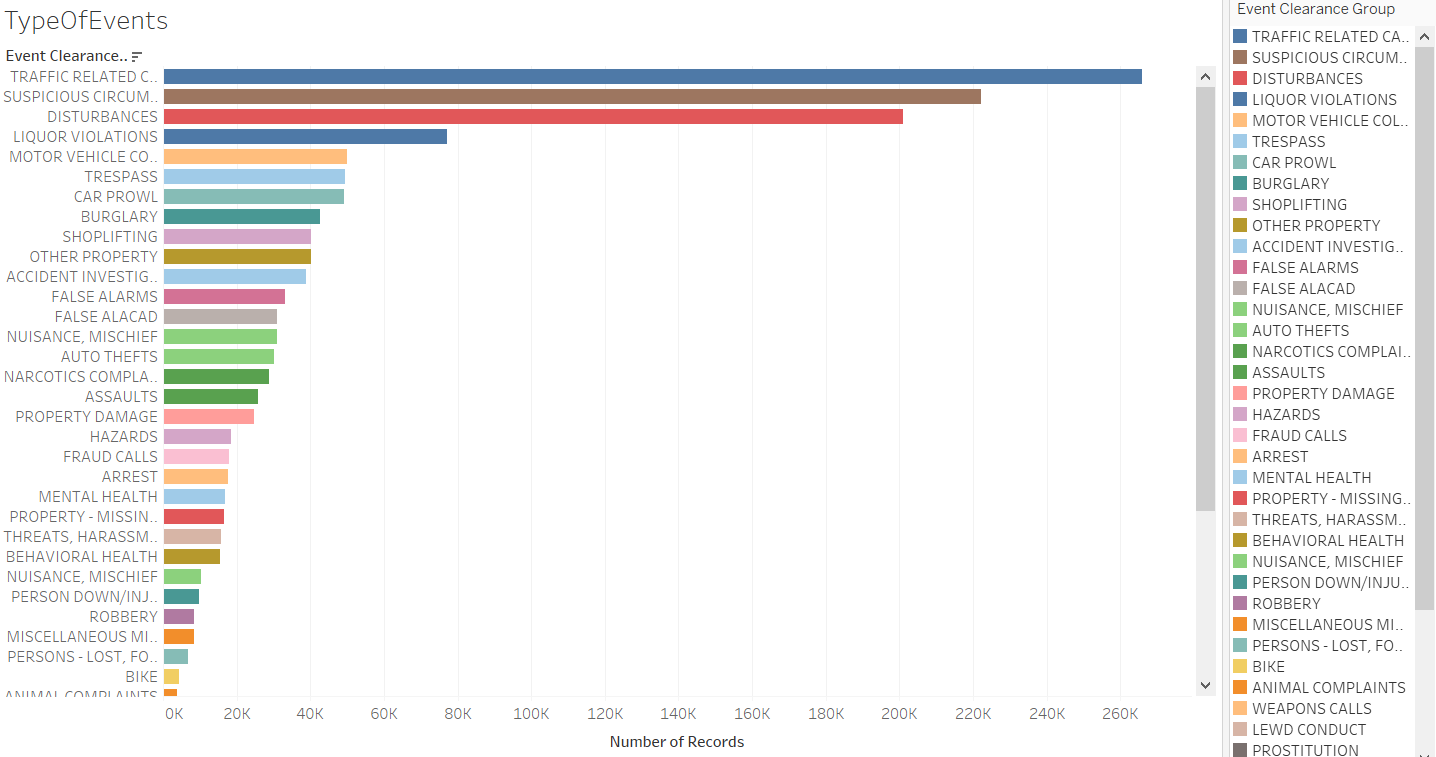
\includegraphics[width=\textwidth]{VisualAnalytics/Assignment2/images/TypeOfEvents.PNG}
    \\\\
        The complete visualization can be accesed via tableu public using the following link:
        \url{https://public.tableau.com/profile/charx#!/vizhome/Seattle911Calls_5/CrimeByZones} under metadata and "TypeOfEvents" tab.
        
\section{Task	2:	Exploring	the	incidents’	geographical	and	temporal	distribution}
    \subsubsection {Do you	see	a	different	spatial	distribution	of	incidents	over	the	different	years?	If	so,	which	are	the	differences	you	found?}
        For this exploration we will be using our "SeatleCrime" Dashboard, incidents are shown here in a 3-way manner first by exploring a map of the city of Seatle using the coordinates of the incidents of our data, then type of events and number of records and finally a distribution of this events over time, event types are ordered by number of incidents in a descending order.
        \\
        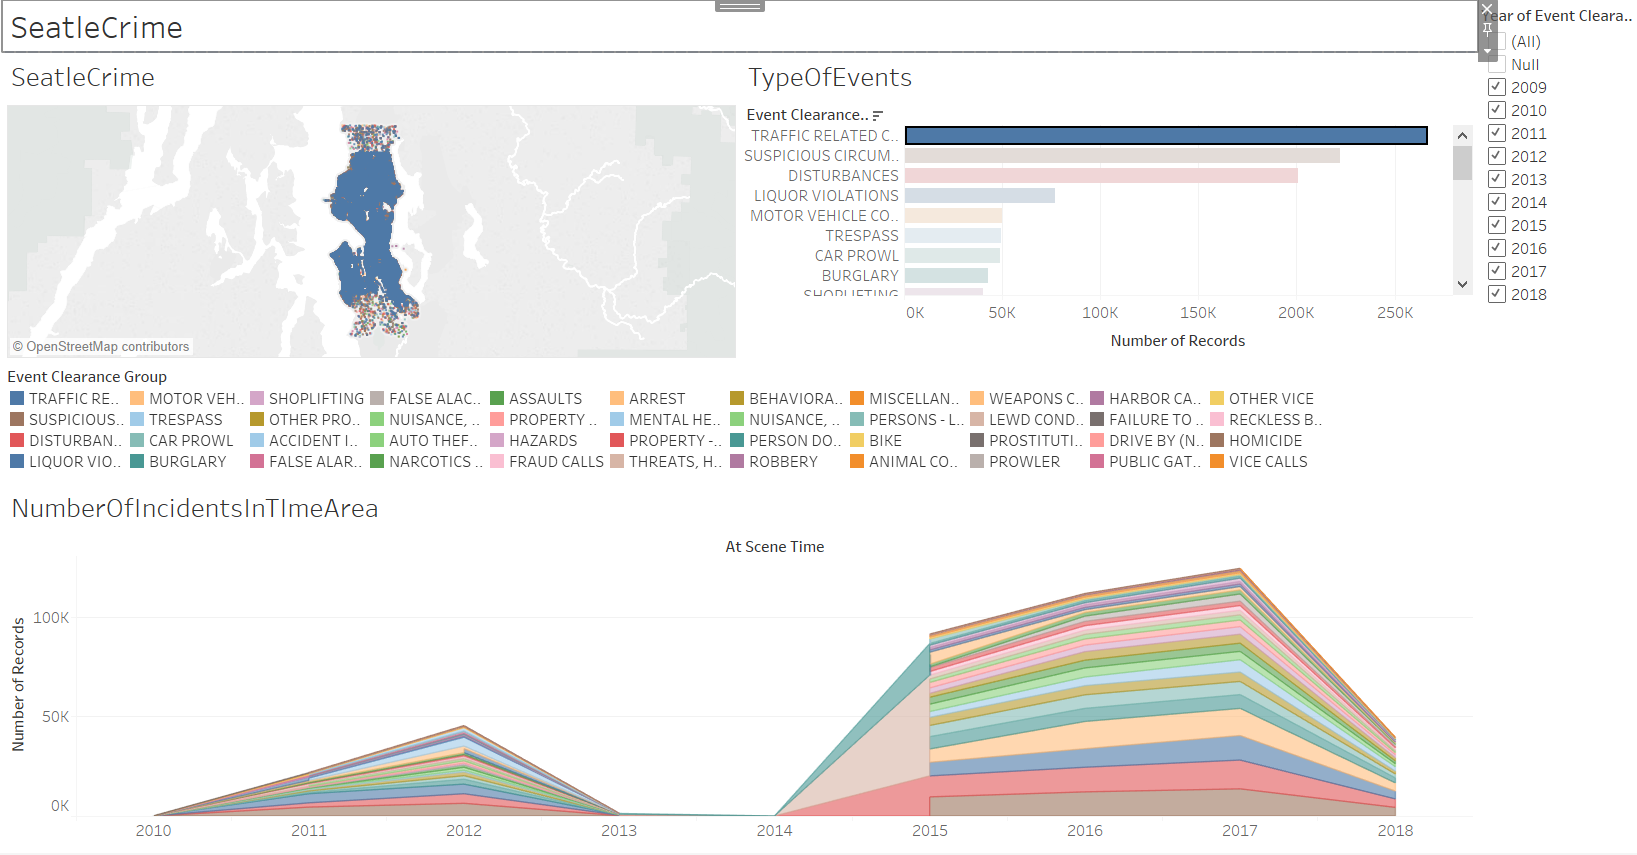
\includegraphics[width=\textwidth]{VisualAnalytics/Assignment2/images/SpatialDistDashboard1.PNG}
        \\
        We can observe a sudden difference with records of the years 2013 and 2014, such records appear to be missing, there is certainly lack of data regarding those years. Next we will use tableaus filtering options of our dashboard to in detail determine how incidents are changing over time, we observe that there has been a steady increase in Seatle's crime numbers, 
        \\
        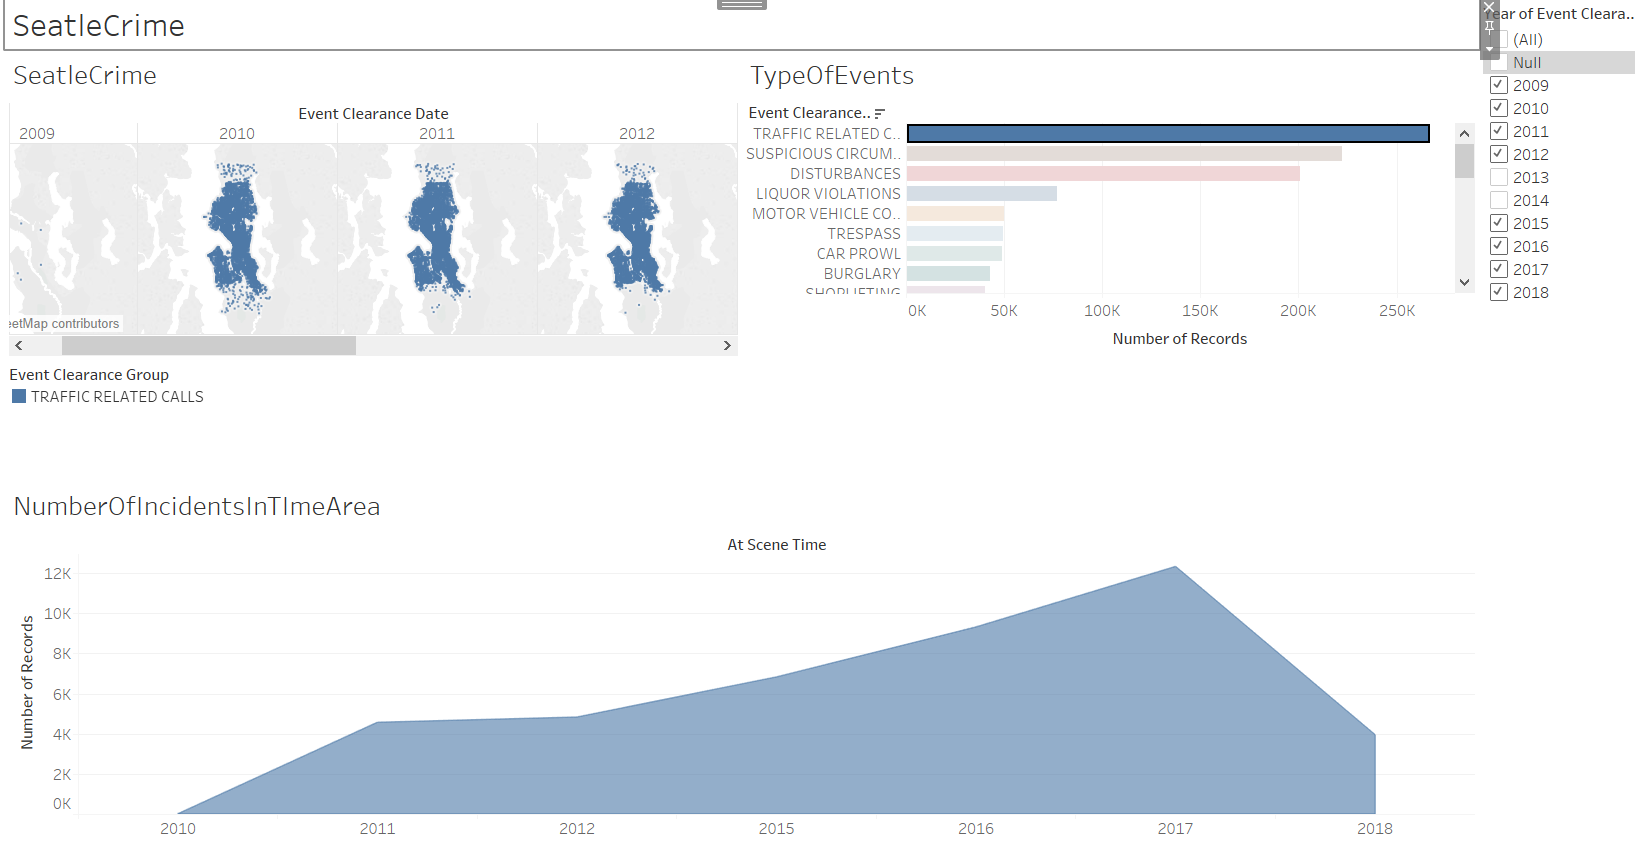
\includegraphics[width=\textwidth]{VisualAnalytics/Assignment2/images/SpatialDistDashboard2.PNG}
        \\
        \url{https://public.tableau.com/profile/charx#!/vizhome/Seattle911Calls_5/SeatleCrime?publish=yes} under metadata and "SeattleCrime" tab.
    \subsection{Are there zones with a consistent low incident density over all years? Are there zones	with a consistent high incident	density	over all years?}
    We are going to be using another dashboard approach this time by plotting a time series of number of records divided by zones in descending order, we can see that zones K, M and E contribute the most to the number of records no matter the year except for 2015 were crime went down, but got back on the rise during 2016.
    \\
    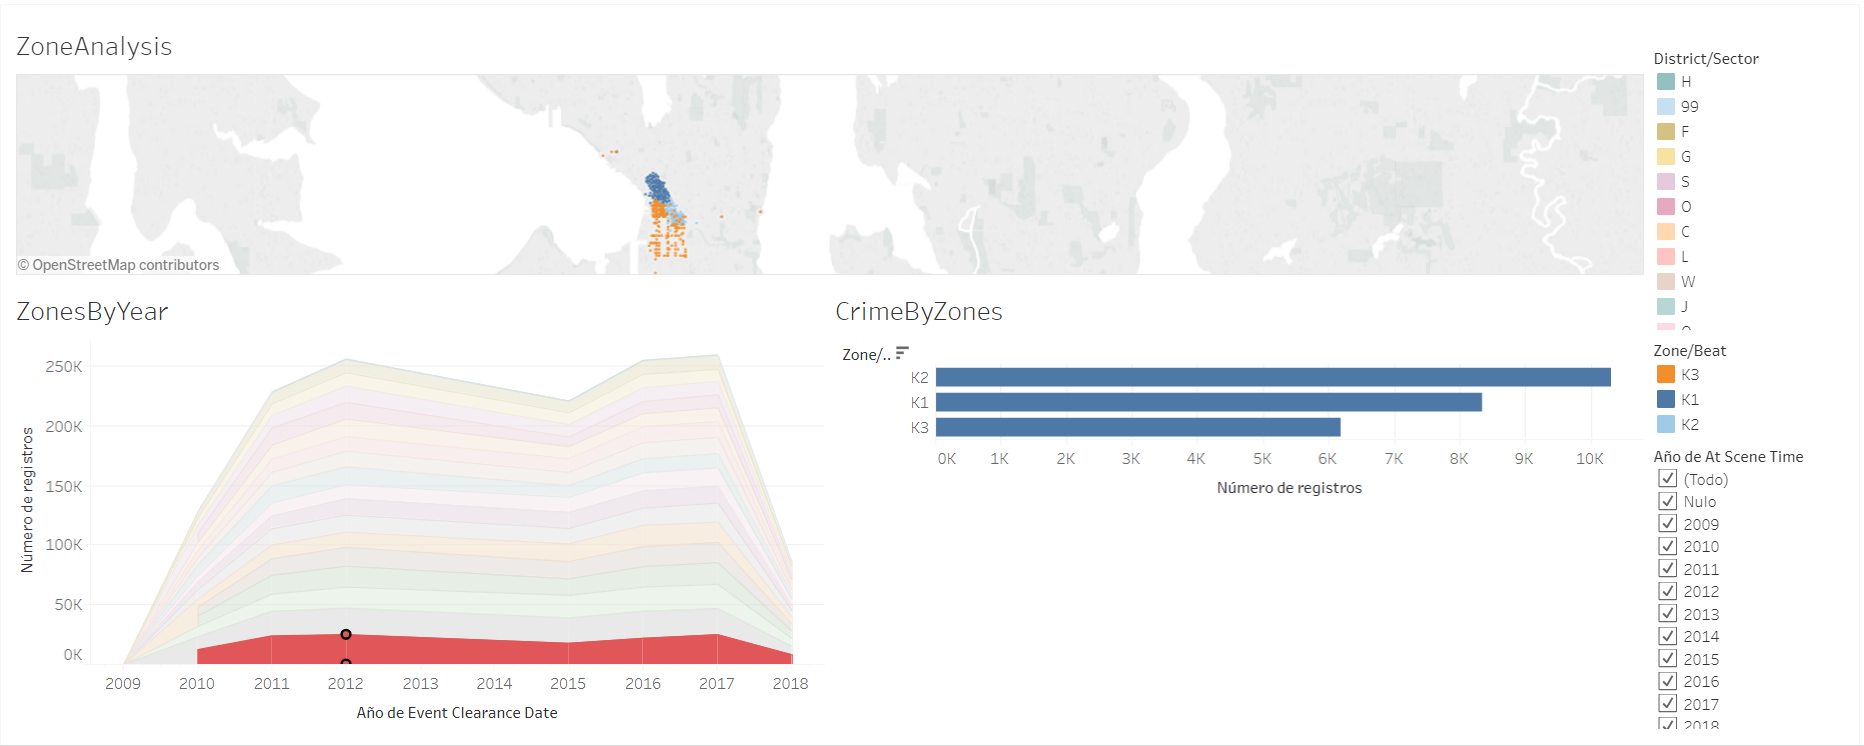
\includegraphics[width=\textwidth]{VisualAnalytics/Assignment2/images/CrimeByZoneDashboard.PNG}
    \\
    We can refer to \url{https://public.tableau.com/profile/charx#!/vizhome/Seattle911Calls_5/CrimeByZone?publish=yes} under metadata and "CrimeByZone" tab
    
\section{Exploring the resolution Speed}
    \subsection{What is the	average	resolution speed to	an incident? Resolution	speed is defined	as the difference between the Event	Clearance Date value (moment when the police closed the file	of	an	incident) and the At Scene Time value (moment	when	the	police	arrived	at	the	scene of the incident).}
    For this task we did a calculation in tableau and created a new calculated field "Response Time" by subtracting "At Scene Time" to "Event Clearence Date" in hours, after this we perform an average and histogram of response time: the average resolution speed is \textbf{1.99} hours, on the histogram of the visualization we observe a fat tailed distribution we are going to change the scale at a logarithm level to obtain a clearer representation of our distribution.
    \\
    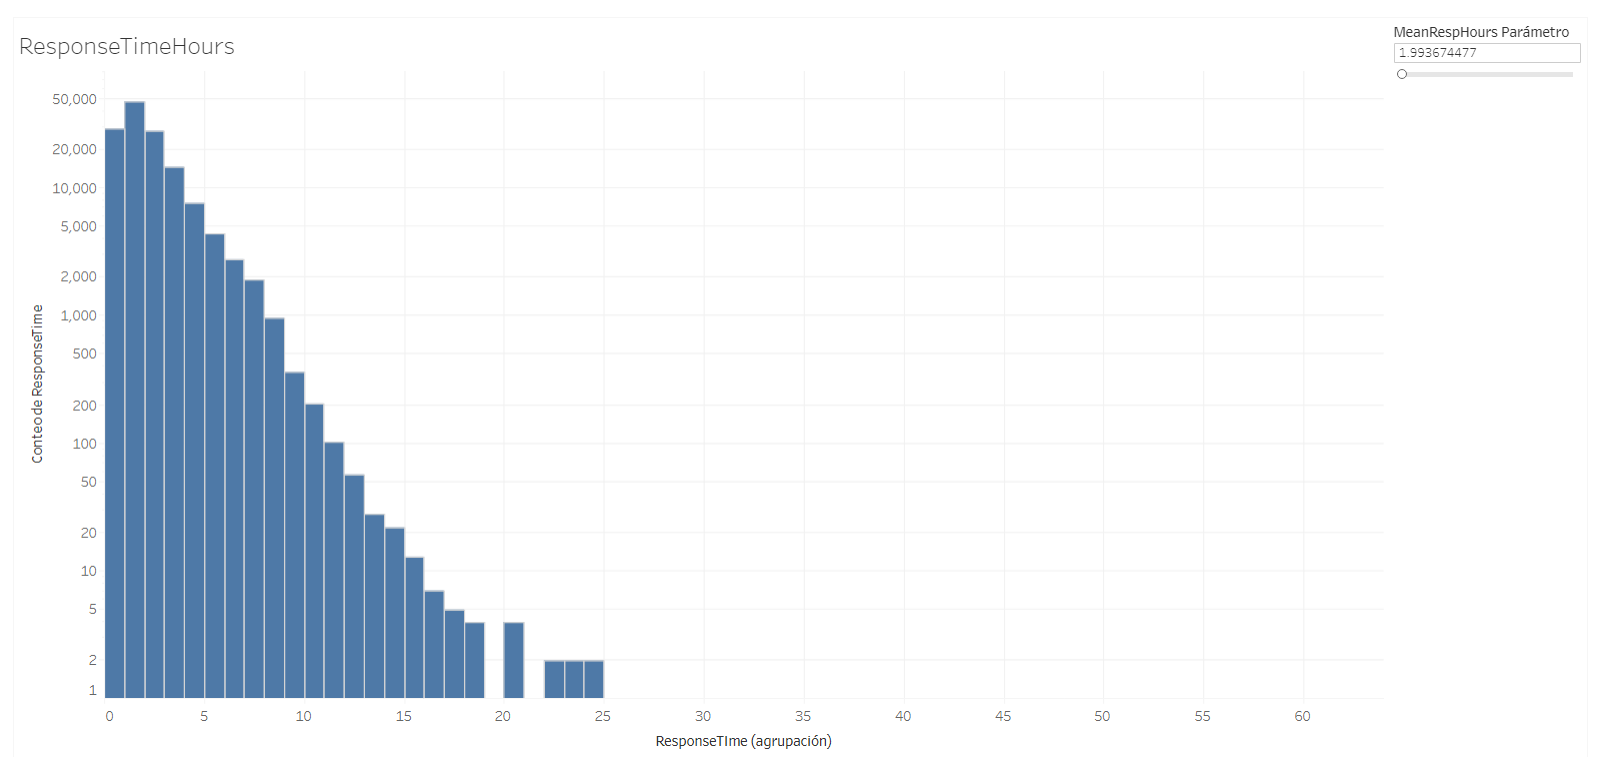
\includegraphics[width=\textwidth]{VisualAnalytics/Assignment2/images/ResponseTimeDist.PNG}
    \\
    We can refer to \url{https://public.tableau.com/profile/charx#!/vizhome/Seattle911Calls_5/ResponseTimeHours} under metadata and "ResponseTimeHours" tab.
    
    \subsection{Are there certain types of incidents having a much lower resolution speed than others? If so,	which are these?}
    For this task we will focus our attention on the sum of resolution speed by the category "Event Clearence Group" after that we will sort the sum of resolution speeds in descending order and obtain that the categories: Motor vehicle collision investigation, suspicious circumstances and disturbances sum the most hours. 
    \\
    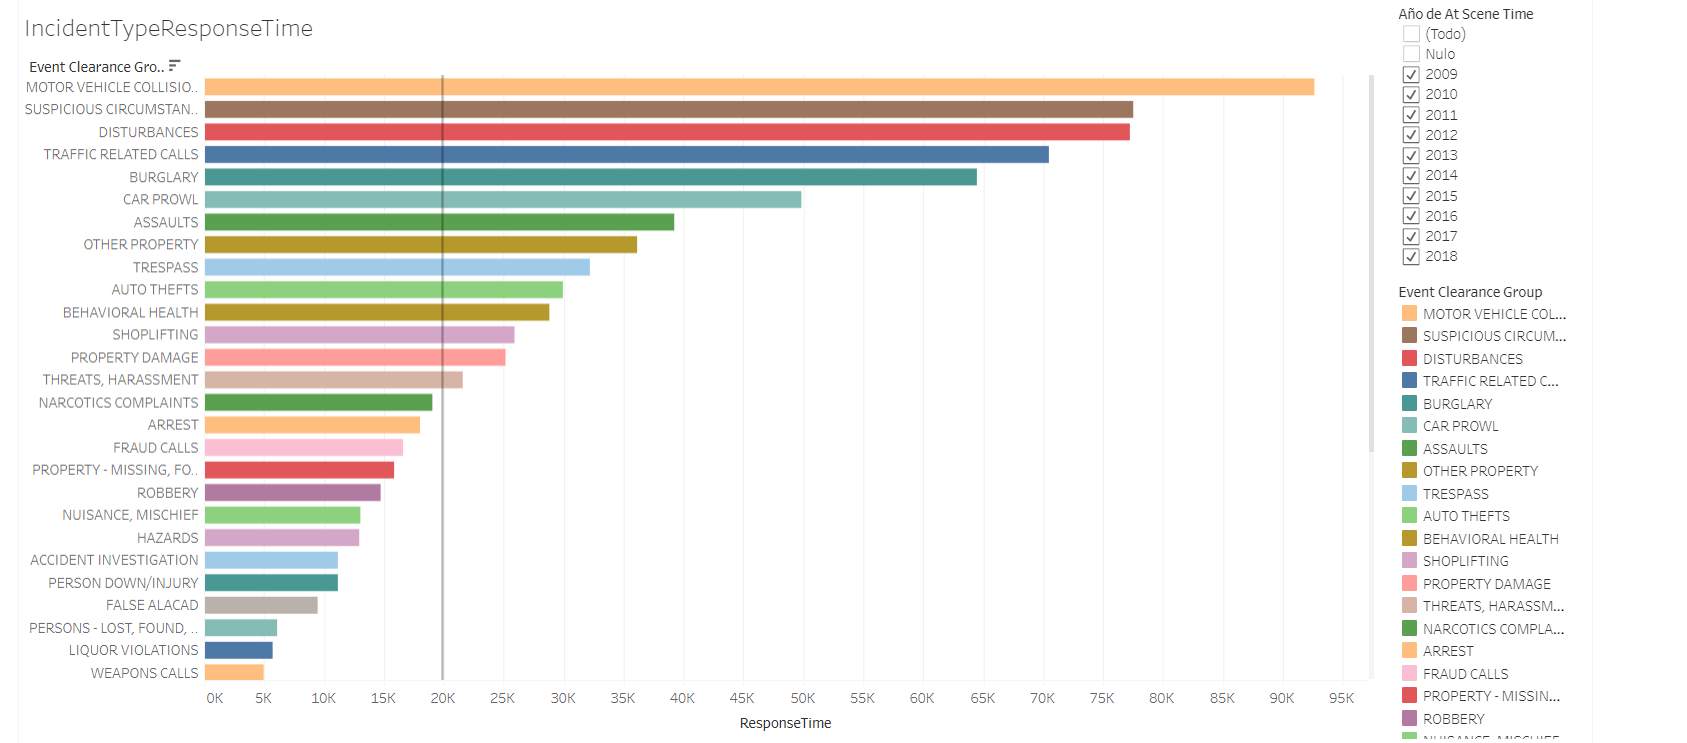
\includegraphics[width=\textwidth]{VisualAnalytics/Assignment2/images/ResponseTimeCategory.PNG}
    \\
    We can refer to \url{https://public.tableau.com/profile/charx#!/vizhome/Seattle911Calls_5/IncidentTypeResponseTime} under metadata and "IncidentTypeResponseTime" tab.
    \subsection{Does the resolution	speed depend on	the	time period	(e.g., year, season	of	the	year)?}
    For this task we did a dashboard presentation approach in order to get a clear vision on the periodicity of response time, we ploted the accumulated response time by quarter T1, T2, T3, T4 to see if there was a variation between each one of them and in fact yes we got a sudden drop in response time for the T2 periods of the year, this shows that there is a dependence on ResponseTime and the time period.
    \\
    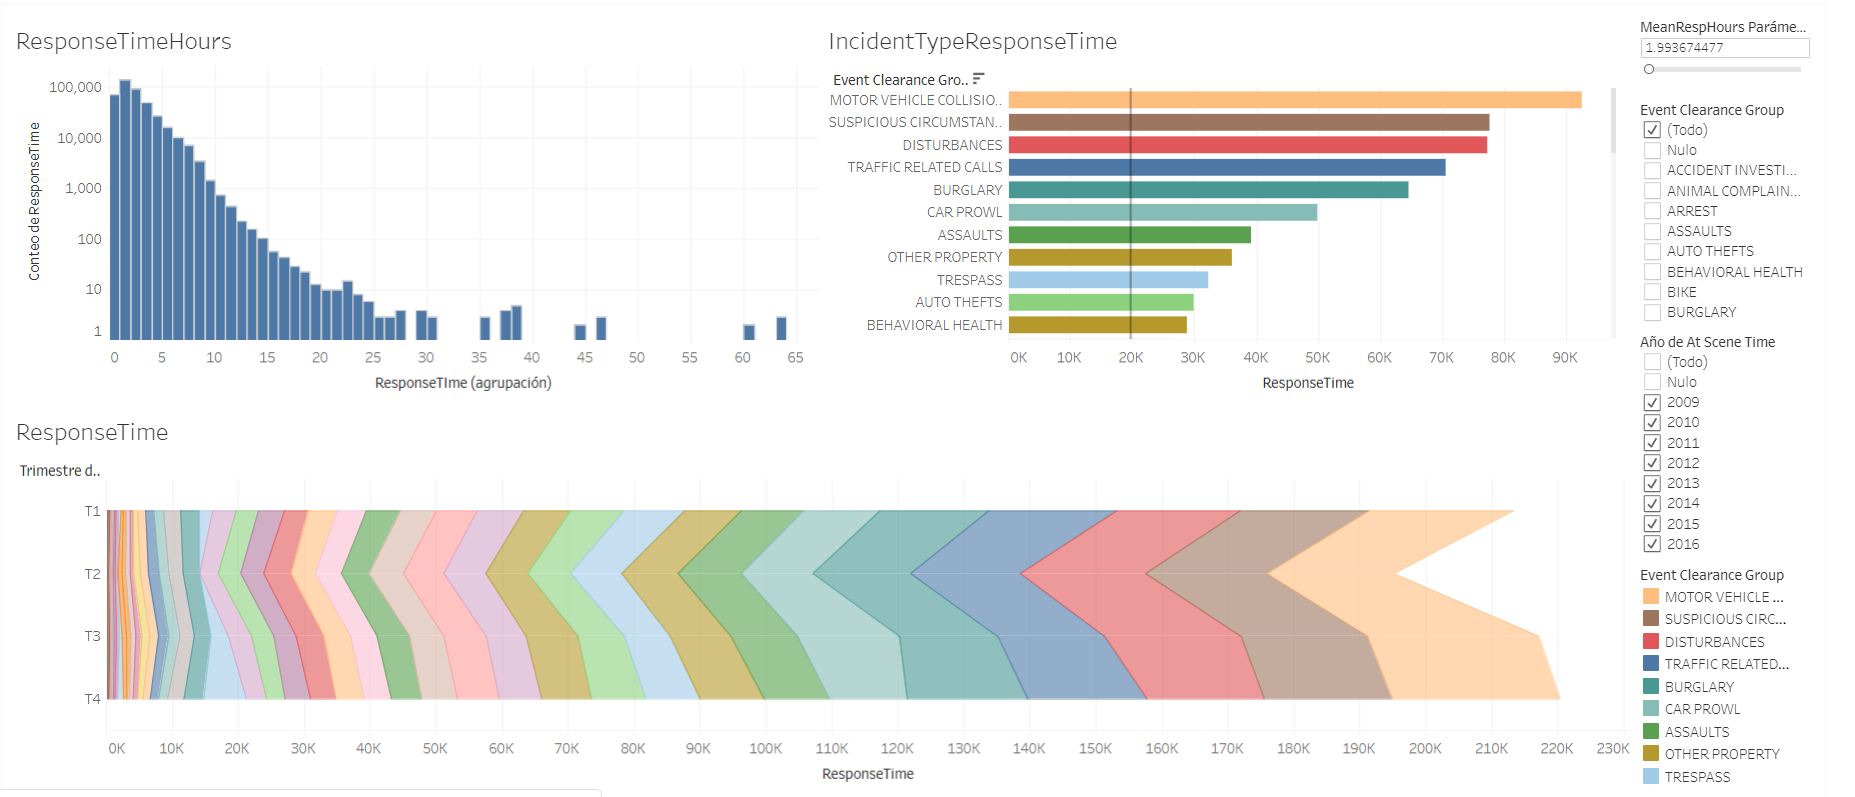
\includegraphics[width=\textwidth]{VisualAnalytics/Assignment2/images/ResponseTimeSeason.PNG}
    \\
    We can refer to \url{https://public.tableau.com/profile/charx#!/vizhome/Seattle911Calls_5/ResolutionSpeed} under metadata and "ResolutionSpeed" tab.
    \section{Exploring the incidents classification}
    \subsection{Incidents have	 two	 types:	 the type of the	incident	 at	 the	moment	it	 was	 reported (Initial	 Type	 Group)	 and	 the	 type	 of	 the	 incident	 after	 it	 has been studied and classified (Event	 Clearance	Group).	Obviously, there should be some kind of correlation of the latter with the former (for instance, incidents reported as robberies are very likely to be also classified finally as robberies). How strong is	this correlation?}
    This task is quite a challenge because it is difficult to visualize the correlation between 2 categorical variables without any other point of reference, so our approach was to make a heat map based on 3 things, the "Initial type Group" and the "Event clearance group" with varying size of squares that indicate the number of reports on each "cross-category". For example a lot of initial group parking violations are categorized as "traffic related calls" on clearence. 
    \\
    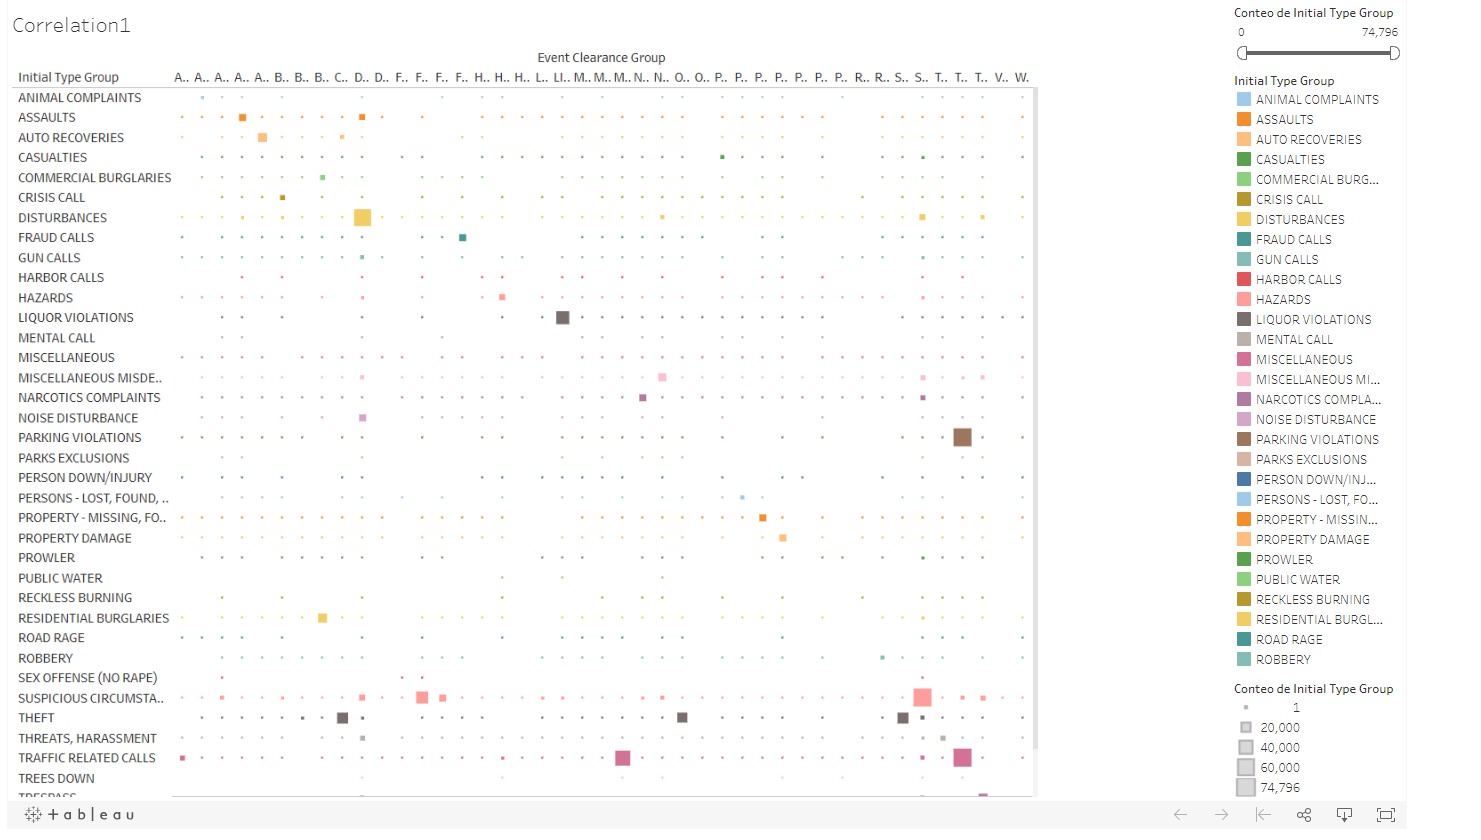
\includegraphics[width=\textwidth]{VisualAnalytics/Assignment2/images/Correlation1.PNG}
    \\
    The complete visualization can be accesed via: \url{https://public.tableau.com/profile/charx#!/vizhome/Seattle911Calls_5/Correlation1?publish=yes} under metadata and "Correlation1" tab.
    
    \subsection{How	do the total number of incidents break down	per	incident reported type (Initial Type Group) and incident resolution type (Event Clearance Group)?}
    Another great way to visualize this question is not to use size because there can be correlation with not a lot of reported incidents but with a color gradient as an indicator of the number of records reported on each "cross-category", now we can see much more clearly that "suspicious circumstances" is reported at initial time a lot but it gets "cleared" into all the categories, and "sex offenses" just lead to "failure to register".
    \\
    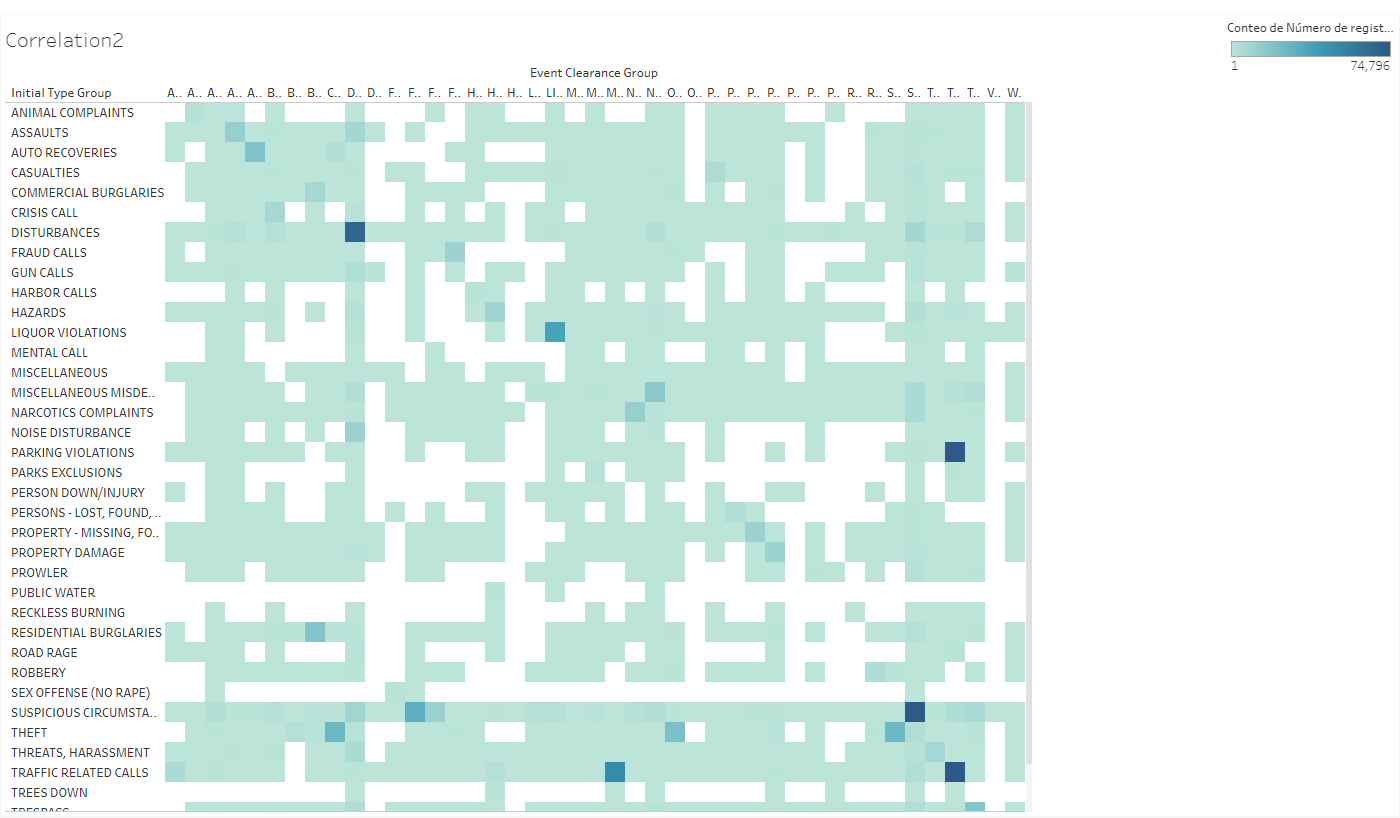
\includegraphics[width=\textwidth]{VisualAnalytics/Assignment2/images/Correlation2.PNG}
    \\
    The complete visualization can be accesed via: \url{https://public.tableau.com/profile/charx#!/vizhome/Seattle911Calls_5/Correlation2?publish=yes} under metadata and "Correlation2" tab.
    \\
    \subsection{How do the total number of incidents break down per incident resolution	 type (Event	Clearance Group) and incident resolution subtype (Event	Clearance Subgroup)?}
    We ploted each "Event Clearance Group" and number of records with "Event clearance sub-group" as a way to color our bar charts, we can see very clearly if one type of incident gets turned into another category at clearance by lookin at the color of the graphs. For example, nearly 1/4 of auto-thefts gets cleared into "auto-recoveries" on clearance.
    \\
    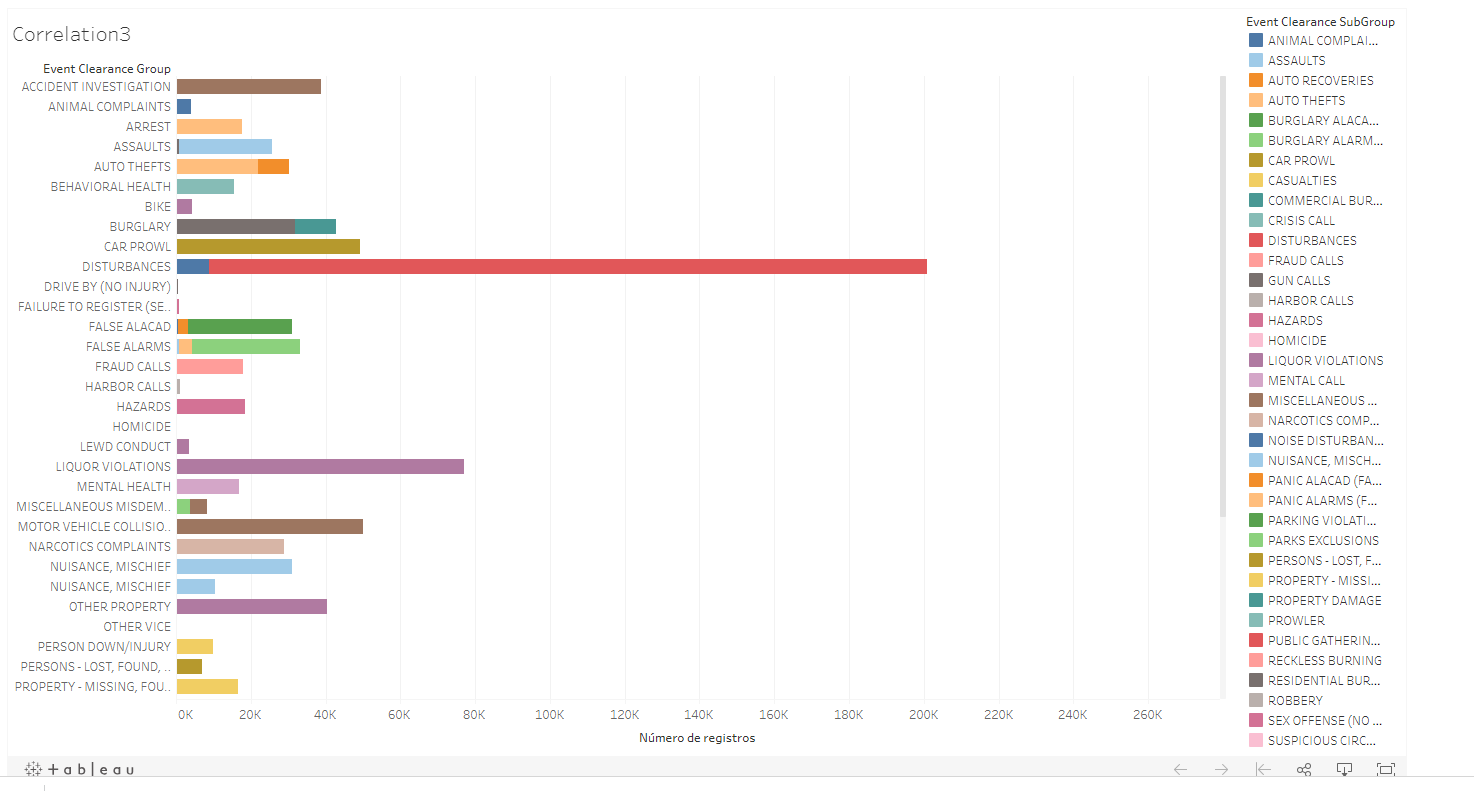
\includegraphics[width=\textwidth]{VisualAnalytics/Assignment2/images/Correlation3.PNG}
    \\
    The complete visualization can be accesed via: \url{https://public.tableau.com/profile/charx#!/vizhome/Seattle911Calls_5/Correlation3?publish=yes} under metadata and "Correlation3" tab.
    \\

    \section{Exploring the incidents temporal distribution}
    
    
\end{document}